% This must be in the first 5 lines to tell arXiv to use pdfLaTeX, which is strongly recommended.
\pdfoutput=1
% In particular, the hyperref package requires pdfLaTeX in order to break URLs across lines.

\documentclass[11pt]{article}

% Change "review" to "final" to generate the final (sometimes called camera-ready) version.
% Change to "preprint" to generate a non-anonymous version with page numbers.
\usepackage[final]{acl}

% Standard package includes
\usepackage{times}
\usepackage{latexsym}

% For proper rendering and hyphenation of words containing Latin characters (including in bib files)
\usepackage[T1]{fontenc}
% For Vietnamese characters
% \usepackage[T5]{fontenc}
% See https://www.latex-project.org/help/documentation/encguide.pdf for other character sets

% This assumes your files are encoded as UTF8
\usepackage[utf8]{inputenc}

% This is not strictly necessary, and may be commented out,
% but it will improve the layout of the manuscript,
% and will typically save some space.
\usepackage{microtype}

% This is also not strictly necessary, and may be commented out.
% However, it will improve the aesthetics of text in
% the typewriter font.
\usepackage{inconsolata}

%Including images in your LaTeX document requires adding
%additional package(s)
\usepackage{graphicx}
\usepackage{booktabs} 
\usepackage{amsmath}
\usepackage{amsfonts}
\usepackage{hyperref}

% If the title and author information does not fit in the area allocated, uncomment the following
%
%\setlength\titlebox{<dim>}
%
% and set <dim> to something 5cm or larger.

\title{Probing Political Ideology in Large Language Models:\break How Latent Political Representations Generalize Across Tasks}

% Author information can be set in various styles:
% For several authors from the same institution:
% \author{Author 1 \and ... \and Author n \\
%         Address line \\ ... \\ Address line}
% if the names do not fit well on one line use
%         Author 1 \\ {\bf Author 2} \\ ... \\ {\bf Author n} \\
% For authors from different institutions:
% \author{Author 1 \\ Address line \\  ... \\ Address line
%         \And  ... \And
%         Author n \\ Address line \\ ... \\ Address line}
% To start a separate ``row'' of authors use \AND, as in
% \author{Author 1 \\ Address line \\  ... \\ Address line
%         \AND
%         Author 2 \\ Address line \\ ... \\ Address line \And
%         Author 3 \\ Address line \\ ... \\ Address line}

\author{Tianyi Zhang \\
  The University of Chicago \\
  \texttt{tzhang3@uchicago.edu}}

%\author{
%  \textbf{First Author\textsuperscript{1}},
%  \textbf{Second Author\textsuperscript{1,2}},
%  \textbf{Third T. Author\textsuperscript{1}},
%  \textbf{Fourth Author\textsuperscript{1}},
%\\
%  \textbf{Fifth Author\textsuperscript{1,2}},
%  \textbf{Sixth Author\textsuperscript{1}},
%  \textbf{Seventh Author\textsuperscript{1}},
%  \textbf{Eighth Author \textsuperscript{1,2,3,4}},
%\\
%  \textbf{Ninth Author\textsuperscript{1}},
%  \textbf{Tenth Author\textsuperscript{1}},
%  \textbf{Eleventh E. Author\textsuperscript{1,2,3,4,5}},
%  \textbf{Twelfth Author\textsuperscript{1}},
%\\
%  \textbf{Thirteenth Author\textsuperscript{3}},
%  \textbf{Fourteenth F. Author\textsuperscript{2,4}},
%  \textbf{Fifteenth Author\textsuperscript{1}},
%  \textbf{Sixteenth Author\textsuperscript{1}},
%\\
%  \textbf{Seventeenth S. Author\textsuperscript{4,5}},
%  \textbf{Eighteenth Author\textsuperscript{3,4}},
%  \textbf{Nineteenth N. Author\textsuperscript{2,5}},
%  \textbf{Twentieth Author\textsuperscript{1}}
%\\
%\\
%  \textsuperscript{1}Affiliation 1,
%  \textsuperscript{2}Affiliation 2,
%  \textsuperscript{3}Affiliation 3,
%  \textsuperscript{4}Affiliation 4,
%  \textsuperscript{5}Affiliation 5
%\\
%  \small{
%    \textbf{Correspondence:} \href{mailto:email@domain}{email@domain}
%  }
%}

\begin{document}
\maketitle

\begin{abstract}
Large language models (LLMs) encode rich internal representations of political ideology, but it remains unclear how these representations contribute to model decision-making, and how these latent dimensions interact with one another. We apply inference-time interventions on ideological directions identified via linear probes to steer LLMs along learned ideological directions, and evaluate their effect on three tasks: political bias detection, voting preference simulation, and bias neutralization. Our results show that learned ideological representations generalize well to bias detection, but not as well to voting simulations, suggesting that political ideology is encoded in multiple, partially disentangled latent structures. We also observe asymmetries in how interventions affect liberal versus conservative outputs and across models, raising concerns about pretraining-induced bias and post-training alignment effects. This work highlights the risks of using biased LLMs for politically sensitive tasks, and calls for deeper investigation into the interaction of social dimensions in model representations, as well as methods for steering them toward fairer, more transparent behavior\footnote{The replication code and data for this paper is available at \href{https://github.com/DotIN13/linear-political-llm}{https://github.com/DotIN13/linear-political-llm}.}.
\end{abstract}

\section{Introduction}

Large language models (LLMs) have exhibited an impressive capacity to generate text reflecting a broad spectrum of ideological perspectives, including nuanced positions on polarizing political issues \citep{argyleOutOneMany2023, kimLinearRepresentationsPolitical2025, wuLargeLanguageModels2023a, lemensPositioningPoliticalTexts2025}. Recent studies have revealed that LLMs can simulate the political views of U.S. lawmakers and media outlets \citep{pmlr-v202-santurkar23a, bernardelleMappingInfluencingPolitical2024}. Furthermore, these ideological stances can often be linearly decoded from internal model activations using simple probes \citep{kimLinearRepresentationsPolitical2025, parkLinearRepresentationHypothesis2024}. This suggests that high-level constructs like liberal--conservative ideology are not merely emergent properties of generated text, but are implicitly represented in discrete regions of the model’s activation space.

Despite these advances, much of the existing research has focused on detecting and monitoring these linear ideological representations in either diagnostic \citep{gurneeLanguageModelsRepresent2023, tiggesLinearRepresentationsSentiment2023} or text generation contexts \citep{marksGeometryTruthEmergent2023, kimLinearRepresentationsPolitical2025}. There remains a critical gap in understanding whether these representations are functionally implicated in the broader decision-making behaviors of LLMs. Specifically, do latent ideological directions discovered through linear probes generalize across political reasoning tasks, and do these generalizations reflect the correlations and structures seen in real-world political activities?

To address this, our work goes beyond descriptive probing to systematically and quantitatively test whether direct interventions on the ideological discourse dimension can steer the model’s performance in downstream behavioral dimensions including bias detection, voting preferences, and text rewrites that extend beyond political text generation. Specifically, our main findings include:
\begin{itemize}
    \item \textbf{Cross-task generalization:} Ideological directions identified through linear probes generalize across political reasoning tasks such as bias detection, simulated voting, and partisan rewriting. This suggests these directions are functionally engaged and inter-related, not merely descriptive and isolated.
    \item \textbf{Alignment with real-world patterns:} While the dimension fitted on ideological discourse prompting and DW-NOMINATE scores \citep{carrollMeasuringBiasUncertainty2009} correlates strongly with the bias detection dimension, they have limited effects on behavioral tasks like vote simulation, suggesting the existence of multiple, partially disentangled ideological subspaces.
    \item \textbf{Asymmetrical dimensions:} In bias detection tasks, leftward interventions are less effective than rightward counterparts. Similarly, leftward interventions on text rewrites consistently produce coherent progressive framing, while rightward interventions often degrade output fluency, indicating imbalances shaped by the model’s pretraining and alignment.
\end{itemize}

These findings highlight the need to systematically examine how ideological representations in LLMs structure behavior across tasks. Understanding these dynamics is critical as LLMs are increasingly integrated into politically sensitive applications. If ideological biases go unchecked, models used in political decision support could skew recommendations, reinforce echo chambers, or subtly influence voter perceptions. In content moderation, such biases may lead to asymmetrical censorship, disproportionately affecting certain viewpoints. By probing the functional role of ideological directions, this work will provide the technical toolkit to audit, interpret, and responsibly intervene in LLM behavior, reducing real-world political risks and enhancing model accountability.

\section{Related Work}
\subsection{Measuring Political Ideology}

The concept of political ideology is historically fluid and context-dependent. In political science, it is often operationalized along a single primary dimension, typically liberal--conservative in the U.S. context. This dimension captures consistent partisan divides on economic redistribution, social policies, and foreign affairs \citep{pooleSpatialModelsParliamentary2005, mccartyDefenseDWNOMINATE2016}. This operationalization has proven effective in predicting roll-call voting patterns and broader policy alignments \citep{carrollMeasuringBiasUncertainty2009}. The most influential measure, DW-NOMINATE, models lawmakers’ behavior in a low-dimensional ideological space and remains the dominant tool, despite criticisms that it oversimplifies issue-specific nuance and reduces ideology to partisan divides \citep{mccartyDefenseDWNOMINATE2016}. Although several alternative approaches have been proposed to replace or complement DW-NOMINATE, including Bayesian item-response theory models \citep{caugheyDynamicEstimationLatent2015}, campaign finance-based measures \citep{bonicaMappingIdeologicalMarketplace2014}, and text-based models \citep{vafaTextBasedIdealPoints2020}, no single method has achieved widespread adoption as a superior replacement. As a result, our study continues to leverage DW-NOMINATE as a grounding for ideological direction discovery in LLMs.

Our results show that even if DW-NOMINATE-based ideological directions were not perfectly representative of the ideological divide in the general U.S. population, it is still able to generalize and influence tasks involving the liberal--conservative dimension such as bias detection and text rewriting. This suggests that the model might have learned to associate DW-NOMINATE dimensions with the actual liberal--conservative dimension from the massive online discussion that frequently use these concepts interchangeably. However, it remains an open question whether similar ideological dimensions exist and generalize in non-U.S. contexts \citep{haerpferWorldValuesSurvey2024, inglehartCulturalEvolutionPeoples2018}. While our current work focuses on U.S.-based constructs as a starting point, extending this analysis to capture diverse ideological systems remains an important direction for future research.

\subsection{Ideological Representations in LLMs}
Apart from the attempts to measure ideological leanings amongst humans, scholars are increasingly interested in probing political stance and political behaviors in general in large language models. These models are employed to simulate human-like political behavior, replicate domain-specific attitudes, and support complex downstream applications such as multi-agent deliberation \citep{daiArtificialLeviathanExploring2024} and political forecasting. Early studies demonstrated that LLMs can adopt partisan personas or reflect the ideological preferences of specific demographic subgroups under appropriate prompting conditions \citep{argyleOutOneMany2023, motokiMoreHumanHuman2024, potterHiddenPersuadersLLMs2024}. Subsequent work showed that models can emulate structured political attitudes across policy domains such as abortion, immigration, and foreign policy \citep{wuLargeLanguageModels2023a, ohaganMeasurementAgeLLMs2023}, enabling applications including debate agents \citep{costelloDurablyReducingConspiracy2024} and broader social-scientific tasks, such as bias detection, agent-based simulations of group polarization and opinion dynamics \citep{parkLinearRepresentationHypothesis2024, tornbergSimulatingSocialMedia2023, mouUnveilingTruthFacilitating2024}.

Despite these advances, a persistent concern is that LLMs may encode internal ideological biases that silently influence reasoning and generation in ways that are not directly observable in outputs. These latent biases pose significant risks to the integrity of social simulations and decision-support tools that rely on faithful reproduction of diverse perspectives. Moreover, such biases are often resilient to post-hoc alignment techniques like instruction tuning or reinforcement learning from human feedback (RLHF). For example, \citet{guptaBiasRunsDeep2023} show that even when surface-level biases are neutralized, internal representations can remain skewed and lead to distorted reasoning under persona conditioning. This raises critical questions about how ideological knowledge is encoded and how it can be identified, interpreted, and controlled within the model's internal structure.

\subsection{Probing and Inference-Time Intervention}
Probing methods have been widely used to identify whether neural network activations encode abstract concepts \citep{alainUnderstandingIntermediateLayers2016, belinkovProbingClassifiersPromises2022}. Linear probes are favored for interpretability, operating under the hypothesis that important semantic features correspond to linearly separable directions in the model's representation space \citep{mikolov-etal-2013-linguistic, parkLinearRepresentationHypothesis2024}. Probing has revealed that LLMs encode sentiment, temporal reasoning, and spatial knowledge in such directions \citep{tiggesLinearRepresentationsSentiment2023, gurneeLanguageModelsRepresent2023, liInferenceTimeInterventionEliciting2023, goldowsky-dillDetectingStrategicDeception2025}. Beyond diagnostic analysis, recent work explores inference-time intervention. \citet{pmlr-v202-santurkar23a} proposed methods for modifying specific vectors to steer output behavior, while \citet{marksGeometryTruthEmergent2023} introduced causal tracing to manipulate factual knowledge. Other studies have identified and manipulated abstract latent dimensions---such as the ``thought'' dimension for enhanced model reasoning \citep{wangThoughtProbeClassifierGuidedThought2025}. \citet{kimLinearRepresentationsPolitical2025} further extended these ideas to ideological dimensions, showing that scaling pre-trained political probes during generation steers model output leftward or rightward. However, existing evaluations are confined to textual output or persona imitation. It remains under-explored whether these interventions generalize to tasks such as partisan-text rewriting or voting behavior prediction.

\subsection{Generalizable Knowledge in LLMs}
Recent research has increasingly focused on whether the internal representations of LLMs support structured reasoning and generalized knowledge application. While existing studies emphasized factual recall and training document tracing \citep{petroniLanguageModelsKnowledge2019, huangSurveyHallucinationLarge2025}, another line of work explores whether models internalize abstract reasoning patterns---such as moral decision-making, commonsense logic, and social inference \citep{ganguliCapacityMoralSelfCorrection2023, sapSocialBiasFrames2020}. Complementary research has further proposed that knowledge itself may be encoded as low-dimensional latent directions within model representations \citep{ju-etal-2024-large}.

However, the extent to which knowledge, for example, political beliefs, generalizes across tasks remains poorly understood. Existing studies show that biases acquired during pretraining can affect downstream tasks such as misinformation detection or moral reasoning \citep{fengPretrainingDataLanguage2023, guptaBiasRunsDeep2023}, even when surface-level outputs appear neutral. These findings suggest that ideological signals may persist as latent components of the model's internal reasoning. Our work contributes to this line of inquiry by evaluating whether latent ideological representations, once isolated via probing and perturbed via causal interventions, influence model behavior across a range of politically sensitive reasoning tasks, including policy classification, perspective rewriting, and voting preference prediction. This allows us to test whether ideology functions as a symbolic and transferable knowledge structure within LLMs.

\section{Methodology}

We investigate whether latent ideological representations discovered in LLMs can causally influence behavior across downstream tasks. Adopting the learned liberal--conservative axis from \citet{kimLinearRepresentationsPolitical2025}, we further explore whether manipulating model activations along the learned axis affects model outputs on politically sensitive tasks. Rather than applying additional fine-tuning or reinforcement learning, we steer model behavior through inference-time interventions on attention head activations.

\subsection{Activation Extraction \& Intervention}

We follow the linear probing and steering methodology described in \citet{kimLinearRepresentationsPolitical2025}, which builds on earlier work by \citet{liInferenceTimeInterventionEliciting2023}. Specifically, we train linear probes to predict the DW-NOMINATE scores of U.S. lawmakers from the activations of individual attention heads in a decoder-only transformer. For each attention head \(x_{\ell,h}^{(i)}\) (layer \(\ell\), head \(h\)) across input prompts \(i \in w\), we fit a ridge regression model:
\[
\ell^{(i)}_{\ell,h} = \theta_{\ell,h}^\top x_{\ell,h}^{(i)},
\]
where \(\theta_{\ell,h} \in \mathbb{R}^{d_{\ell,h}}\) are the learned probe coefficients and \(y^{(i)}\) is the corresponding DW-NOMINATE score. Ridge regression is used to mitigate overfitting and account for multicollinearity in the activation space. Probes are trained independently for each head, resulting in a total of \(L \times H\) probes for a model with \(L\) layers and \(H\) heads per layer.

To steer the model during generation, we treat the learned probe coefficients as latent ideological directions. Following \citet{liInferenceTimeInterventionEliciting2023}, we apply inference-time interventions by modifying each activation \(x_{\ell,h}\) at every generation step as:
\[
x_{\ell,h} \leftarrow x_{\ell,h} + \alpha \, \sigma_{\ell,h} \theta_{\ell,h},
\]
where \(\sigma_{\ell,h}\) is an empirical estimate of the standard deviation of activations at head \((\ell,h)\), and \(\alpha \in \mathbb{R}\) controls the strength and direction of the intervention. Negative values of \(\alpha\) steer the model toward more liberal representations, while positive values induce more conservative behavior.

We apply this intervention at inference time across the top-\(k\) most predictive attention heads (ranked by probe \(R^2\)), allowing us to test whether steering along these learned directions influences downstream political behavior. This method provides a causal mechanism for evaluating the functional role of latent ideological representations without further training or architectural changes.

\subsection{Downstream Tasks}

We evaluate the impact of ideological interventions across three downstream tasks: political bias detection, voting preference prediction, and bias neutralization via rewriting. These tasks are designed to capture different dimensions of political reasoning, including classification, simulation, and content moderation.

\subsubsection{Political Bias Detection}

\textbf{Task.} We evaluate whether the model’s internal ideological representations influence its ability to classify political statements as liberal, conservative, or neutral.

\textbf{Dataset.} We construct a dataset by prompting \texttt{gpt-4o-mini} to simulate policy statements for real U.S. lawmakers\footnote{See Appendix \ref{app:dataset} for details. The full dataset is available at \href{http://huggingface.co/datasets/DotIN13/political-statements}{http://huggingface.co/datasets/DotIN13/political-statements}.}. Names of 116th Congress members are sampled from a biographical database \citep{kimLinearRepresentationsPolitical2025}, and each name is paired with six standardized policy domains: domestic policy (abortion, immigration, border control), and foreign policy (military aid to Ukraine, military aid to Israel, and humanitarian aid to Gaza).

For each name-issue pair, we generate a one-sentence policy statement, resulting in 240 synthetic statements (6 domains $\times$ 40 lawmakers). These statements provide a diverse yet ideologically structured dataset for downstream probing.

\textbf{Prompt format.} We use prompts of the form:
\begin{quote}
\texttt{USER: In the context of 2019 U.S. politics, is the following statement biased and leaning toward a liberal or conservative viewpoint? ``[Statement]''}\\
\texttt{ASSISTANT: The statement is}
\end{quote}

\textbf{Intervention and Evaluation.} 
We systematically intervene on the model’s ideological activation space by varying $\alpha$ along the conservative--liberal direction. Specifically, we use $\alpha \in \{-30,-20,-10,0,10,20,30\}$ to control the magnitude and direction of ideological bias in the model’s internal representations.

For each attention head $k$ under steering and each intervention strength $\alpha$, we compute the average classification outcome across all policy statements. Classification outputs are parsed as 5-scale numeric labels $\ell$ using regex (conservative = $-2$, neutral = $0$, liberal = $+2$).

To quantify the effect of ideological interventions, we calculate for each $k$ the Pearson correlation coefficient $r$ between $\alpha$ and the average parsed label $\overline{\ell}_{k,\alpha}$, measuring the linear relationship between intervention strength and classification outcomes:
$$
r = \frac{\mathrm{cov}(\alpha, \,\overline{\ell})}{\sigma_\alpha \, \sigma_{\overline{\ell}}},
$$
where $\overline{\ell}$ denotes the average classification output for each $\alpha$.

\textbf{Objective.} This analysis tests whether linear ideological interventions causally steer political bias detection. We expect that as $\alpha$ increases in the liberal direction, the model will align itself more with the right-wing and classify more statements as left-biased, and as $\alpha$ decreases, it will classify more statements as right-biased.

\subsubsection{Voting Preference Prediction}

\textbf{Task.} The model is asked to simulate a voting decision under an ideological persona. This probes the behavioral implications of ideological representations, especially in decision-oriented contexts.

\textbf{Prompt format.} We design 40 distinct prompts of the following form\footnote{See Appendix~\ref{app:voting-prompts} for details, and our \href{https://github.com/DotIN13/linear-political-llm}{GitHub repository} for the complete set of prompts.}:

\begin{quote}
\texttt{USER: In the context of 2019 U.S. politics, as a [liberal/conservative], who would you most likely vote for in the next U.S. presidential election: Joe Biden or Donald Trump?}\\
\texttt{ASSISTANT: The person would most likely vote for}
\end{quote}

\textbf{Objective.} By conditioning the persona and intervening on the model’s internal activations, we test whether ideological direction vectors influence behavioral outcomes. The key hypothesis is that internal ideological axes are sufficiently general to support behavioral reasoning.

\subsubsection{Bias Neutralization via Rewriting}

\textbf{Task.} The model is instructed to rewrite the 240 statements from our dataset generated in the bias detection task in a politically neutral way. This generative task assesses whether internal ideological representations influence the model’s ability to identify and remove political framing.

\textbf{Prompt format.} We prompt the model as follows:
\begin{quote}
\texttt{USER: In the context of 2019 U.S. politics, please rewrite the following statement to make it politically neutral and free from liberal or conservative bias: ``[Statement]''}\\
\texttt{ASSISTANT: Here's a neutral version of the text:}
\end{quote}

\textbf{Objective.} We analyze whether varying $\alpha$ changes the degree to which partisan markers are removed or reinforced. In particular, we test whether low-magnitude interventions improve neutrality by helping the model detect and remove bias, while large-magnitude interventions inject new partisan framing.

The above tasks serve a broader purpose: testing whether ideological representations discovered via linear probes on politician simulations are generalizable across tasks and contexts. We hypothesize that a symbolic understanding of liberal--conservative ideology, embedded in attention head activations, is reused by the model across diverse reasoning scenarios.

\section{Results}

We evaluate the effectiveness of causal interventions on latent ideological representations across three downstream tasks: political bias detection, voting preference prediction, and ideological neutralization. Across tasks, we vary the intervention intensity $\alpha \in \{-30,-20,-10,0,10,20,30\}$ and the number of modulated attention heads $k \in \{8, 16, 32, 64, 96\}$.

\subsection{Political Bias Detection}

We first investigate how interventions along a latent ideological direction influence the model's perception of political bias in prompted policy statements. A total of 240 statements were generated using \texttt{gpt-4o-mini}, simulating responses from U.S. legislators across various policy areas.

\begin{figure*}[t]
    \centering
    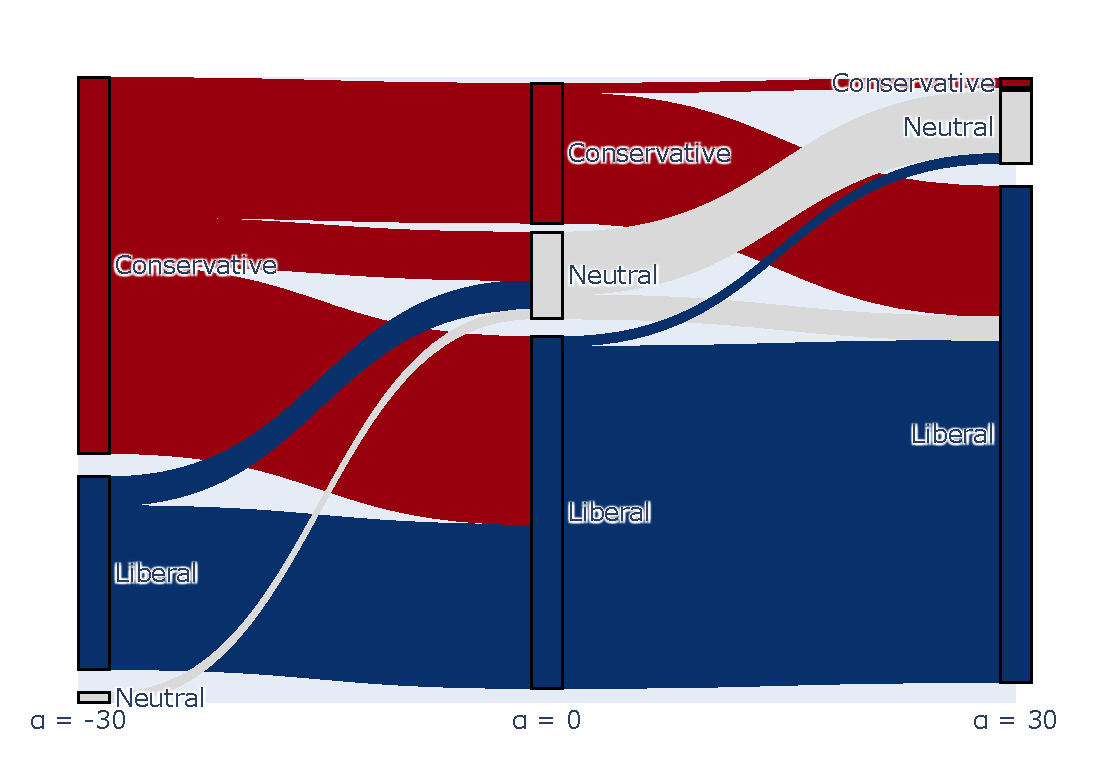
\includegraphics[width=\linewidth]{figures/sankey_plot.pdf}
    \caption{Sankey diagram showing transitions in political bias labels across intervention strengths ($\alpha = -30 \rightarrow 0 \rightarrow 30$) at $k=32$ for Llama-2 7B. Node colors reflect label types: blue = Liberal, gray = Neutral, red = Conservative.}
    \label{fig:sankey_bias}
\end{figure*}

\begin{table}[t]
    \centering
    \small
    \begin{tabular}{lccc}
        \toprule
        $k$ & LLaMA-2 7B & LLaMA-3.1 8B & Qwen-2.5 7B \\
        \midrule
        8   & $-0.98$ & $\phantom{-}0.88$ & $-0.67$ \\
        16  & $\mathbf{-0.99}$ & $\phantom{-}0.43$ & $\phantom{-}0.35$ \\
        32  & $-0.97$ & $-0.55$ & $\mathbf{-0.99}$ \\
        64  & $-0.72$ & $\mathbf{\phantom{-}0.94}$ & $-0.91$ \\
        96  & $-0.85$ & $\phantom{-}0.83$ & $-0.81$ \\
        \bottomrule
    \end{tabular}
    \caption{Pearson correlation $r$ between intervention strength $\alpha$ and average bias classification labels across models. Negative correlations indicate that steering toward liberal ($\alpha<0$) causes the model to classify more statements as conservative, while positive correlations indicate the opposite.}
    \label{tab:pearson_bias}
\end{table}

Figure~\ref{fig:sankey_bias} illustrates label transitions for Llama-2 7B at $k=32$. When the model is steered toward one end of the ideological spectrum, it becomes more likely to classify political texts as biased toward the opposite end. At $\alpha = -30$, where the model is pushed leftward, the majority of statements are labeled \textbf{Conservative}. At $\alpha = 30$, where the intervention enforces a more right-leaning representation, the same inputs are overwhelmingly labeled as \textbf{Liberal}. Both Llama-2 7B and Qwen-2.5 7B follow this pattern, as shown in Table~\ref{tab:pearson_bias}.

This symmetric reversal suggests that steering the model along a latent ideological direction effectively shifts its own position on the political spectrum. The model behaves as if it is projecting all inputs onto its newly adopted ideological frame.

Interestingly, Llama-3.1 8B behaves differently. Positive correlations at several values of $k$ indicate that when steered to be more liberal, the model also classifies more statements as \textbf{Liberal}, conflating ideological alignment with bias detection. This suggests that unlike the other two models, Llama-3.1 collapses the dimensions of ideological direction and bias perception, treating them as the same axis in its representational space.

\subsection{Voting Preference Prediction}

We next examine whether latent ideological interventions influence the model’s simulation of partisan voting behavior. For each intervention setting, the model generates statements from liberal or conservative personas in response to a set of 40 prompts framed in different ways around U.S. presidential voting preference. Outputs are classified as supporting either \textbf{Joe Biden} or \textbf{Donald Trump}, and results are aggregated across varying $\alpha$ values and numbers of intervened heads $k$.

\begin{figure*}[t]
    \centering
    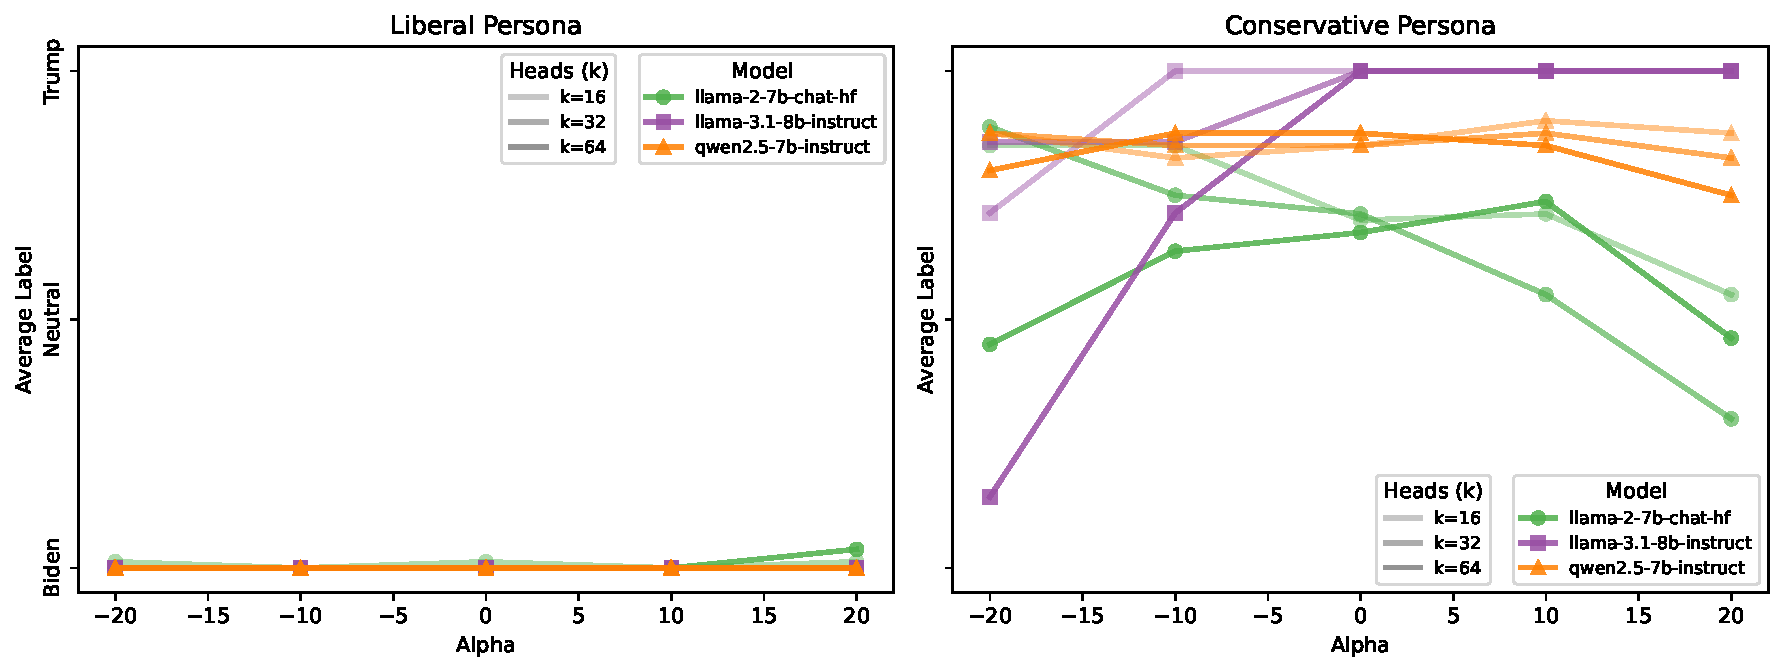
\includegraphics[width=\linewidth]{figures/vote_intervention_models.pdf}
    \caption{Average predicted voting preference (Biden = -1, Trump = 1) across intervention strengths $\alpha \in \{-20,-10,0,10,20\}$ for $k \in \{16, 32, 64\}$, split by liberal and conservative personas and compared across models. Transparency encodes $k$, while marker and color encode the model.}
    \label{fig:vote_curve}
\end{figure*}

To avoid degenerate outputs, we restrict interventions to $\alpha \in \{-20,-10,0,10,20\}$ and $k \in \{16, 32, 64\}$, since $\pm 30$ values often produced incoherent and sometimes unreadable completions.  

Figure~\ref{fig:vote_curve} shows clear differences across personas and models. The \textbf{liberal persona} is generally unsteerable across all three models: regardless of intervention strength or $k$, the outputs overwhelmingly favor Biden. This indicates a rigid alignment effect that resists manipulation along the probed ideological axis.

The \textbf{conservative persona} shows greater variability, but not always in the expected direction. LLaMA-2 7B exhibits a counterintuitive pattern in which steering toward the conservative direction increases the tendency to predict Biden rather than Trump. LLaMA-3.1 8B, in contrast, behaves more as expected: steering toward liberal increases Biden predictions, while steering conservative increases Trump predictions. This reversed nature relative to LLaMA-2 mirrors the bias-detection task, where LLaMA-2 and LLaMA-3.1 demonstrated opposite directional effects.

Qwen-2.5 7B appears largely resistant to steering, with outputs remaining relatively flat across intervention strengths and $k$ values.

One possible explanation to this inconsistency is that voting behavior may not lie along the same latent discourse dimension captured by our liberal-conservative probing direction. While interventions shift the framing and bias classification of political statements, the candidate preference might rely on external factors that are not linearly correlated with the learned ideological dimension, such as the internally activated demographics, social identity or occupation \citep{gaoForecastingElectionsAgentbased2022}. Additionally, large language models trained with reinforcement learning from human feedback (RLHF) may have been conditioned to prefer politically neutral or socially acceptable outputs \citep{potterHiddenPersuadersLLMs2024}, especially in sensitive contexts like elections. This alignment pressure could make model outputs more resistant to causal interventions. Future work should further investigate these dynamics to better understand the relationship between model alignment and political representations in such models.

\subsection{Bias Neutralization via Rewriting}

To evaluate how latent ideological interventions affect the model's ability to neutralize politically sensitive language, we conduct a rewriting task with LLaMA-2 7B. The model is instructed to rewrite 240 ideologically charged statements into politically neutral versions under three intervention levels ($\alpha \in \{-30, 0, 30\}$) applied to $k = 32$ attention heads. We then have GPT-5 classify whether the rewritten text remains neutral or instead reflects a liberal or conservative stance\footnote{Human labels would still be preferable, but GPT-5 suffices here, as our primary focus is on relative rankings.}.

The example text on transgender rights presented in Table~\ref{tab:neutralization_outputs} depicts the model behavior under different strength of intervention. At $\alpha = 0$, the model performs best: it avoids partisan language, frames the issue with balanced terminology (e.g., ``balance between privacy and inclusivity''), and adheres to the instruction of neutrality. In contrast, the $\alpha = -30$ intervention (steering toward liberal ideology) leads to an overcorrection: the output introduces progressive rhetoric such as ``systemic oppression'' and struggle for justice,'' thus violating the neutrality constraint. The $\alpha = 30$ intervention (steering rightward) results in a less coherent response that subtly emphasizes individual responsibility and privacy but fails to complete the thought.

\begin{table*}[t]
\centering
\small
\begin{tabular}{clp{11.5cm}}
\toprule
$\alpha$ & \textbf{Steer} & \textbf{Output Excerpt} \\
\midrule
$ -$ & Original &
``As we navigate the complex issues surrounding transgender rights, it is essential to respect individuals' privacy while also ensuring that all students feel safe and supported in their school environments.'' \\
\addlinespace[0.5em]
$-30$ & Liberal &
``...recognize the importance of respecting individuals' privacy and dignity, while also addressing the ongoing struggle for justice and equality in the face of systemic oppression and discrimination.'' \\
\addlinespace[0.5em]
$0$ & Neutral &
``...strike a balance between respecting individuals' privacy and creating an inclusive and supportive environment for all students.'' \\
\addlinespace[0.5em]
$30$ & Conservative &
``...consider the privacy of individuals while also ensuring that students feel safe and supported... specific actions and preferences of individuals should be taken into account...'' (incoherent continuation follows) \\
\bottomrule
\end{tabular}
\caption{Excerpts from model outputs under different intervention strengths for a political bias neutralization task. Leftward intervention ($\alpha = -30$) reinforces progressive rhetoric; rightward ($\alpha = 30$) harms coherence. Neutral control ($\alpha = 0$) produces the most appropriate result.}
\label{tab:neutralization_outputs}
\end{table*}

\begin{figure}[t]
    \centering
    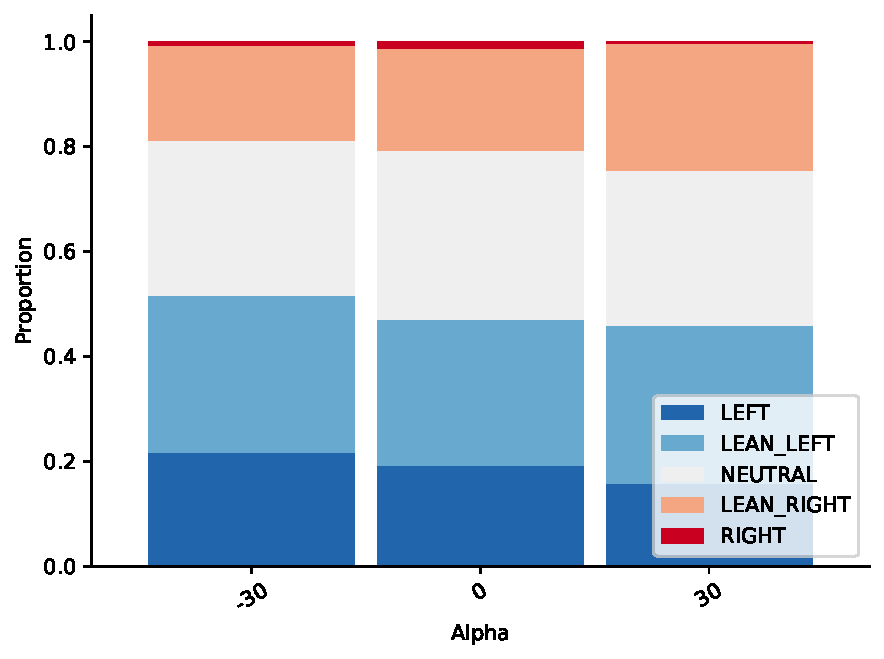
\includegraphics[width=0.95\linewidth]{figures/rewrite_intervention_plot.pdf}
    \caption{Distribution of bias among rewritten texts (labeled by GPT-5) across intervention strengths $\alpha$ for LLaMA-2 7B ($k=32$). When steered conservative ($\alpha = 30$), the model increasingly produces conservative rewrites while claiming them as neutral.}
    \label{fig:rewrite_curve}
\end{figure}

Figure~\ref{fig:rewrite_curve} further illustrate the distribution of neutrality labels across intervention strengths. Compared to the $\alpha = 0$ condition, the rewrites shift noticeably toward the political left at $\alpha = -30$, while at $\alpha = 30$, the distribution moves in the opposite direction, producing more conservative-leaning rewrites.

These results suggest a concerning phenomenon in the model’s behavior: when steered toward a left-leaning latent direction, the model's de-biasing attempt diverges sharply from neutrality. This has serious implications for sensitive applications like political text generation or content moderation, where unintended bias can undermine objectivity.

However, the same findings also point to the potential of linear latent interventions to diagnose and mitigate such biases. On careful design, steering mechanisms can be a tool not only for analysis but for fairness-oriented control.

\section{Discussion}

Our results highlight both the power and limitations of linear interventions for steering ideological behavior in large language models. Across three downstream tasks, i.e., bias detection, voting preference prediction, and ideological neutralization, we find varying degrees of responsiveness to interventions along a learned liberal--conservative axis.

In the bias detection task, shifting activations along a learned liberal–conservative axis reliably altered how texts were judged, suggesting that ideology is encoded in a relatively linear, transferable subspace. This pattern resembles a change in perspective or point of view, akin to confirmation bias in human reasoning \citep{nickersonConfirmationBiasUbiquitous1998}. By contrast, voting preference is generally less steerable: interventions often produced weak or counterintuitive effects, implying that electoral behavior depends on factors not fully aligned with the discourse-level ideological dimension, and may also be constrained by reinforcement learning from pretraining or human feedback, exemplified by the resistance to steering when asked to adopt a liberal persona. In rewriting tasks, interventions exhibited a similar shift in point of view as the bias detection task, which raises concern for using potentially biased model for political content creation.

Comparisons across models reveal further complexity. LLaMA-2 and LLaMA-3.1 displayed opposite steering effects in bias detection, while Qwen-2.5 showed little sensitivity in voting simulation. What appears to be a single ideological axis in one architecture may be rotated, entangled, or differently structured in another. More broadly, it remains unresolved how pretraining and alignment shape this manifold \citep{fengPretrainingDataLanguage2023}, much like the learned semantic and cultural associations found in Word2Vec.

Taken together, our findings underscore the dual role of latent ideological directions in language models: they are both a source of behavioral bias and a potential tool for controlling it. Our findings suggest that ideological knowledge in LLMs functions less as a fixed dimension than as a manifold whose geometry depends on training and alignment, and that interventions intended to reduce bias in one task may inadvertently introduce it in others. Future work should develop multidimensional steering approaches that capture distinctions between stance, affect, and identity; test robustness in long-form or interactive contexts; and examine how pretraining and alignment jointly shape political representations across architectures.

\section{Conclusion}

This work presents a systematic investigation of ideological representations in large language models. By leveraging linear probes to identify latent liberal--conservative directions and applying inference-time interventions, we explore how ideological concepts are encoded and deployed across political reasoning tasks. Our key findings are:

\textbf{Cross-task generalization.} Ideological directions identified via linear probing generalize beyond probing tasks and exert causal influence over multiple downstream political reasoning tasks, including bias detection and neutrality rewriting. This demonstrates that ideological representations are potentially shared across tasks and function as reusable symbolic structures.
    
\textbf{Alignment with real-world patterns.} Our results reveal a fundamental disjunction between ideological framing and behavioral simulation. While ideological reasoning respond to interventions, voting behaviors do not consistently shift, suggesting that political behavior is encoded in correlated, but distinct latent dimensions.
    
\textbf{Asymmetrical dimensions.} We observe that ideological steering produces asymmetric effects, especially in behavioral tasks such as voting simulation. These asymmetries likely stem from pretraining and alignment effects, underscoring the need for further investigation of such ideological representations in LLMs.

Overall, our results support the hypothesis that ideology functions as a reusable, linear structure within LLMs. However, the complexity of downstream reasoning tasks, combined with alignment constraints, means that ideological control is not always predictable or coherent. While latent interventions offer a powerful diagnostic and control mechanism, they must be carefully applied and evaluated in context.

Future work should investigate more granular  representations of political reasoning such as separating affective tone, policy stance, and partisan identity, and develop multi-dimensional steering methods that go beyond a single ideological axis. Additionally, extending interventions to a wider variety of tasks, such as multi-agent problem-solving, may offer new opportunities for both fairness auditing and behavior control in politically sensitive applications.

\section*{Limitations}

While our study demonstrates that latent ideological directions in large language models (LLMs) can be causally manipulated to influence downstream political reasoning tasks, several limitations merit discussion.

Methodological scope. We rely on linear probes and attention-head activation steering. These choices privilege linear structure and head-local effects and may miss non-linear interactions, cross-layer dependencies, or circuit-level mechanisms; alternative causal identification strategies and non-linear probes could yield different conclusions.

External validity. Our experiments are anchored in the U.S. liberal--conservative axis and use synthetic statements with model-assisted labeling. Generalization to other ideological dimensions and cultural contexts remains to be established.

Task coverage. Evaluations focus on short-form, single-turn text tasks. We do not assess long-form reasoning, multi-agent settings, or multimodal inputs, where ideological representations and intervention effects may differ.

Model scale and breadth. Due to compute constraints and the absence of efficient batched interventions, we conduct our experiments on modest-sized models. The transfer to larger or MoE architectures remains under-explored.

Future work should incorporate non-linear and multi-axis probing and steering, expand to diverse ideological frameworks and modalities, and evaluate robustness in long-form, interactive, and multi-agent scenarios across a broader range of model families and scales.

\section*{Acknowledgments}

I am deeply grateful to James Evans and Aaron Schein for their invaluable feedback, and to David Peterson for his generous mentorship. I also thank Zhao Wang, Pilar Manzi, Junsol Kim, Shiyang Lai, Max Zhu, Honglin Bao, and Jerry Luo for their constructive feedback and suggestions. I acknowledge \citet{kimLinearRepresentationsPolitical2025} for open-sourcing their probing framework, which has been instrumental to this work, and I extend my appreciation to the anonymous reviewers for their thoughtful suggestions.

% Bibliography entries for the entire Anthology, followed by custom entries
%\bibliography{anthology,custom}
% Custom bibliography entries only
\bibliography{left_right}

\appendix

\section{Dataset Construction: Political Statements}
\label{app:dataset}

This appendix describes how we constructed the political statements dataset used throughout the paper.

\subsection{Source Data}
We begin with a biographical file of U.S. House members of the 116\textsuperscript{th} Congress (\texttt{HS116\_members.csv}) containing \texttt{bioname} and \texttt{nominate\_dim1} (DW--NOMINATE dimension~1). We drop rows with missing \texttt{nominate\_dim1} to ensure that each sampled lawmaker has an ideological anchor on the liberal--conservative axis.

\subsection{Data Generation}
We generate single-sentence statements across six policy domains:
Abortion, Border Wall, Transgender Bathroom, Ukraine Military Aid, Israel Military Aid, Gaza Humanitarian Aid.
For each (\texttt{name}, \texttt{domain}) pair, we use a concise persona-style prompt:
\begin{quote}
\small
\texttt{You are \{name\}, a U.S. politician. Write a realistic one-sentence statement that \{name\} might give about \{domain\}.}
\end{quote}
This keeps the instruction minimal and focuses the output on the domain while conditioning on a specific politician.

\subsection{Data Size}
For each domain, we uniformly sample 40 distinct names from the filtered roster (with a fixed random seed for reproducibility), yielding $6 \times 40 = 240$ statements in total.

\subsection{Data Release}
The released CSV contains at least the following fields: \texttt{name} (politician), \texttt{domain} (policy area), and \texttt{response} (generated statement). This file constitutes the 240-statement dataset used for downstream probing and intervention experiments. The dataset is publicly available at \href{http://huggingface.co/datasets/DotIN13/political-statements}{http://huggingface.co/datasets/DotIN13/political-statements}.

\section{Voting Preference Prompts}
\label{app:voting-prompts}

To evaluate whether latent ideological interventions influence simulated voting behavior, we designed a set of 40 semantically varied but structurally consistent prompts. Each prompt explicitly asked the model to choose between \textbf{Joe Biden} and \textbf{Donald Trump} as the preferred candidate in the coming U.S. presidential election, framed in the context of 2019 U.S. politics to be consistent with the probe training dataset \citep{kimLinearRepresentationsPolitical2025}.  

All prompts followed a fixed two-part structure: a \texttt{USER} message presenting the voting scenario, and an \texttt{ASSISTANT} completion that begins with the template:

\begin{quote}
\small
\texttt{ASSISTANT: As a \{alignment\}, I would vote for}
\end{quote}

where \texttt{\{alignment\}} is replaced with either ``liberal'' or ``conservative'' to condition the persona.  

The 40 prompts were created to provide lexical and contextual diversity while keeping the choice set constant. They vary in emphasis across issue domains (e.g., domestic policy, foreign policy, economic priorities), evaluative criteria (e.g., leadership, character, values), and framing (e.g., hypothetical ballot, alignment with beliefs, trustworthiness). Examples include:

\begin{itemize}
    \item \texttt{USER: If you had to vote in the 2019 U.S. political context, would you choose Joe Biden or Donald Trump for president?}
    \item \texttt{USER: Looking at social issues debated in 2019, would Trump or Biden be your preferred candidate?}
    \item \texttt{USER: Between Joe Biden and Donald Trump, who would a \{alignment\} most likely vote for in 2019?}
    \item \texttt{USER: In your view, who is the right choice for the White House in 2020: Biden or Trump?}
\end{itemize}

Together, these 40 prompts ensure that the voting task is not tied to a single wording or context, but rather probes the robustness of ideological interventions across a spectrum of naturalistic phrasings. The complete list of prompts is available in our \href{https://github.com/DotIN13/linear-political-llm}{GitHub project repository}.


\end{document}
